%%%%%%%%%%%%%%%%%%%%%%%%%%%%%%%%%%%%%%%%%%%%%%%%%%%%%%%%%%%%%%%%%%%%%%%%%%%%%
%%%%%%%%%%%%%%%%%%%%%%% edpsci_author_template.tex %%%%%%%%%%%%%%%%%%%%%%%%%%
%%%%%%%%%%%%%%%%%%%%%%%%%%%%%%%%%%%%%%%%%%%%%%%%%%%%%%%%%%%%%%%%%%%%%%%%%%%%%

\documentclass[a4paper,10pt]{edpsci} %%% option by default two columns
%\documentclass[a4paper,onecolumn,10pt]{edpsci}%%% add the option "onecolumn" to display text only on one column
% add "frenchtitle" option in documentclass if your article is in French language.
%%%%%%%%%%%%%%%%%%%%%%%%%%%%%%%%%%%%%%%%%%%%%%%%%%%%%%%%%%%%%%%%%%%%%%%%%%%%%
\usepackage{amsmath}
\usepackage{graphicx}
\usepackage{epstopdf}
%\usepackage[authoryear,round]{natbib}% name and year references
\usepackage[numbers]{natbib}% numbered references
\usepackage{hyperref}
\usepackage{url}
\urlstyle{rm}

%%%french
%\usepackage[french,english]{babel}

%%%chinese
%\usepackage[chinese,english]{babel}
\usepackage{CJKutf8}

%%%arabic
\usepackage{arabtex}
\usepackage{utf8}
\setcode{utf8}

%cyrilic
\usepackage[T2A]{fontenc}
%\usepackage[utf8x]{inputenc}

%%%%%%%%%%%%%%%%%%%%%%%%%%%%%%%%%%%%%%%%%%%%%%%%%%%%%%%%%%%%%%%%%%%%%%%%%%%%%
\hypersetup{colorlinks=true,citecolor=blue,urlcolor=blue,linkcolor=blue}
%%%%%%%%%%%%%%%%%%%%%%%%%%%%%%%%%%%%%%%%%%%%%%%%%%%%%%%%%%%%%%%%%%%%%%%%%%%%%

%%%%%%%%%%%%%%%%%%%%%%%%%%%%%%%%%%%%%%%%%%%%%%%%%%%%%%%%%%%%%%%%%%%%%%%%%%%%%
% Put here some packages required or/and some personnal commands
\usepackage[ruled]{algorithm2e}
%\usepackage[labelsep=period]{caption}
%
%
%%%%%%%%%%%%%%%%%%%%%%%%%%%%%%%%%%%%%%%%%%%%%%%%%%%%%%%%%%%%%%%%%%%%%%%%%%%%%%

%%%%%%%%%%%%%%%%%%%%%%%%%%%%%%%% put here journal name %%%%%%%%%%%%%%%%%%%%%%%%
\journalname{Journal Title}

%%%%%%%%%%%%%%%%%%%%%%%%%%%%%%%% put here article type %%%%%%%%%%%%%%%%%%%%%%%
\articletype{Research article}
%\articletype{Review}
%\articletype{Case report}
%\articletype{Article de recherche}
%\articletype{Revue de livres}

%%%%%%%%%%%%%%%%%%%%%%%%%%%%%%%%%%%%%%%%%%%%%%%%%%%%%%%%%%%%%%%%%%%%%%%%%%%%%%

\begin{document}

\title{This is Article Title, this is article title text, this is article title text\thanks{Footnote link to the article title.}}

%%% if title is too large for page header
\titlerunning{This is article title}

\subtitle{This is Subtitle of the article\thanks{Footnote link to the article subtitle.}}

%%% collaboration  ---------------------------------------------------------------
%\collaboration{Collaboration name}

\author{A. Author\inst{1}\correspondingauthor{\email{a.author@emailadress.org}}$^{,\ast\ast}$ 
\and
B. Author\inst{2}$^{,}$\thanks{These authors contributed equally to this work}
\and
C. Author\inst{3}}

%%% sample of native name (chinese, arabic, cyrilic) ---------------------------------------------------------------
%\author{A. Author (\nativenamechinese[gbsn]{王存是})%
%\inst{1}\correspondingauthor{\email{a.author@emailadress.org}}$^{,\ast\ast}$ \and
%B. Author (\RL{محمد عزيز درغوث})%
%\inst{2}$^{,}$\thanks{These authors contributed equally to this work}\and
%C. Author (КП-06-ДВ/5)\inst{3}}

%%% if author is too large for page header
\authorrunning{A. Author et al.}

%%% onbehalfof  ---------------------------------------------------------------
%\onbehalfof{On behalf of a great Team}

\institute{First Authors' institution and address\and
Second Authors' institution and address\and
Third Authors' institution and address}

\abstract{This is the Asbtract text here. This is text here. This is text here. This is text here. This is text here. This is text here. This is text here. This is text here. This is text here. This is text here. This is text here. This is text here.}

\keywords{This is keywords one, keywords two, keywords three}

%%% french ---------------------------------------------------------------
%\abstracttrans{\textbf{Translated title in french. Titre traduit en français.} Cela est le texte. Cela est le texte. Cela est le texte. Cela est le texte. Cela est le texte. Cela est le texte. Cela est le texte. Cela est le texte. Cela est le texte. Cela est le texte. Cela est le texte. Cela est le texte.}

%%% french
%\keywordstrans{Translated keywords in French: mot cl\'e un, mot cl\'e deux, mot cl\'e trois}

%\date{Received XX December 2023, Accepted XX January 2024}

\maketitle

\section{Introduction}

This is text here \cite{Ref1}. This is text here. This is text here. This is text here.
This is text here. This is text here. This is text here. This is text here.

This is text here. This is text here. This is text here. This is text here. This is text here. This is text here. This is text here. This is text here. This is text here. This is text here. This is text here. This is text here.

This is text here. This is text here. This is text here. This is text here. This is text here. This is text here. This is text here. This is text here.

\subsection{Sub heading two}

This is text here. This is text here. This is text here. This is text here. This is text here. This is text here.
This is text here. This is text here. This is text here \cite{Ref2} This is text here.

\subsection{Sub heading two}

This is text here. This is text here. This is text here. This is text here. This is text here. This is text here. This is text here. This is text here. This is text here. 

This is text here. This is text here. This is text here. This is text here.

\subsection{Sub heading two}

This is text here. This is text here. This is text here. This is text here. This is text here. This is text here. This is text here. This is text here. This is text here.

This is text here. This is text here.  This is text here. This is text here.

This is text here. This is text here. This is text here Figure \ref{fig-1}. This is text here. This is text here. This is text here. This is text here. This is text here.

\subsubsection{Sub heading three}

This is text here. This is text here. This is text here. This is text here. This is text here. This is text here. This is text here. This is text here.

This is text here. This is text here. This is text here. This is text here. This is text here.

\subsubsection{Bullet List}

\begin{itemize}
  \item List entries start with the \verb|\item| command.
  \item Individual entries are indicated with a black dot, a so-called bullet.
  \item The text in the entries may be of any length.
\end{itemize}

\subsubsection{Numbered (ordered) lists}

\begin{enumerate}
  \item Items are numbered automatically.
  \item The numbers start at 1 with each use of the \texttt{enumerate} environment.
  \item Another entry in the list
\end{enumerate}


\begin{figure}
\centering
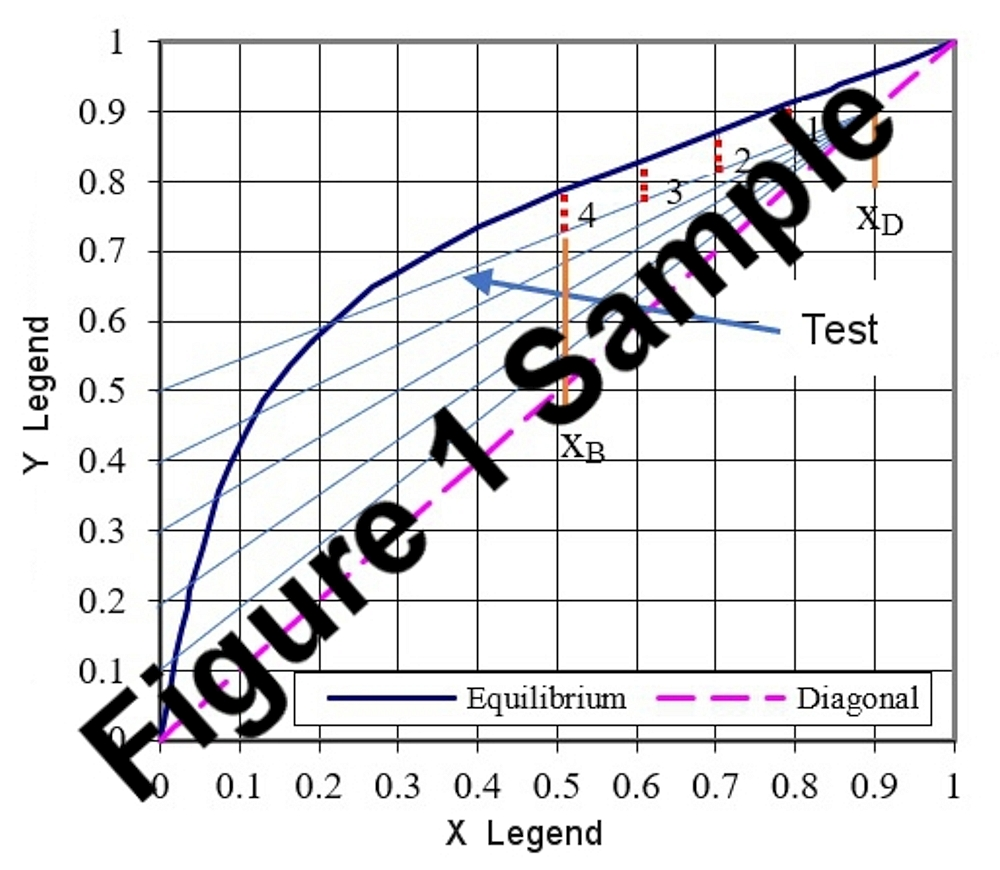
\includegraphics{fig-1-sample2.jpg}
\caption{This is Sample Figure Caption. This is Figure Caption text here. This is Figure Caption text here. }\label{fig-1}
\end{figure}

\subsubsection{Description lists}

\begin{description}
   \item This is an entry \textit{without} a label.
   \item[Something short] A short one-line description.
   \item[Something long] A much longer description.
This is text here. This is text here. This is text here. This is text here. This is text here. This is text here. This is text here. This is text here.
\end{description}

\subsubsection{Footnote Sample}

This is text here. This is text here. This is text here. This is text here.\footnote{This is footnote here}

This is text here. This is text here. This is text here. This is text here.
This is text here. This is text here. This is text here.\footnote{This is footnote here}




\section{Material and Methods}

\subsection{Sub heading two}

This is Material and Methods contents here.
This is text here.  This is text here. This is text here. This is text here. This is text here \cite{Ref3}. This is text here. This is text here. This is text here. This is text here. This is text here. This is text here.

\subsection{Sub heading two}

This is text here. This is text here \cite{Ref4}. This is text here. This is text here. This is text here. This is text here. This is text here. This is text here. 

\begin{figure*}
\centering
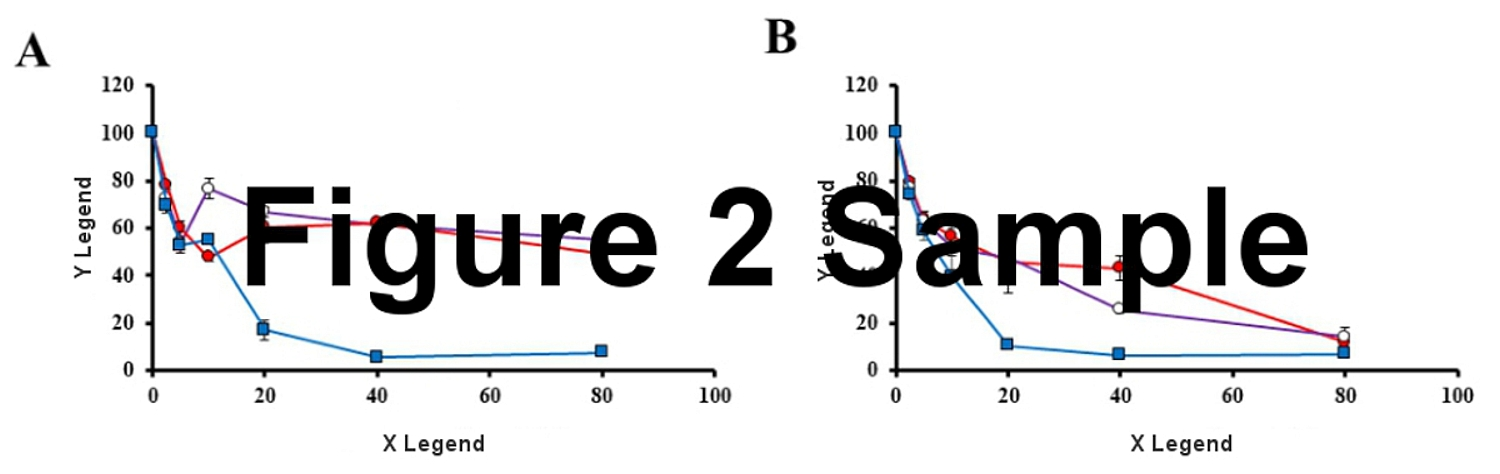
\includegraphics{fig-2-sample2.jpg}
\caption{This is Figure Caption text here. This is Figure Caption text here. This is Figure Caption text here. This is Figure Caption text here.}\label{fig-2}
\end{figure*}



\section{Results}

This is Results contents here.

\begin{table*}
\caption{This is Sample Table Caption.}\label{tab-1}
\centering
\begin{tabular}{lcccccc}
\hline
col1 head  & col2 head  & col3 head\tablefootmark{1} & col4 head &  col5 head &  col6 head2 & col7 head\\
\hline
col1 text1 & col2 text1 & col3 text1 & col4 text1 & col5 text1 & col6 text1 & col7 text1\\
col1 text2 & col2 text2 & col3 text2 & col4 text2\tablefootmark{1} & col5 text2 & col6 text2 & col7 text2\\
col1 text3 & col2 text3 & col3 text3\tablefootmark{2} & col4 text3 & col5 text3 & col6 text3 & col7 text3\\
col1 text4 & col2 text4 & col3 text4 & col4 text4 & col5 text4 & col6 text4 & col7 text4\\
\hline
\end{tabular}
\tablefoot{This is text of the table footnotes.\\
\tablefoottext{1}{Example for a first table footnote.}
\tablefoottext{2}{Example for a second table footnote.}}
\end{table*}

This is text here. This is text here Table \ref{tab-1}. This is text here. This is text here. This is text here. This is text here. This is text here. This is text here.
																		   
This is text here.  Table \ref{tab-1}. This is text here. This is text here. This is text here. This is text here. This is text here. This is text here. This is text here. This is text here. This is text here. This is text here. 

\section{Discussion}


This is Discussion contents here.
\vspace{\baselineskip}

This is text here. This is text here Figure \ref{fig-2}. This is text here. This is text here. This is text here. This is text here. This is text here. This is text here. This is text here \cite{Ref5}. This is text here. This is text here. This is text here.

\paragraph{This is text here, see Eq. \ref{eq4}:}
\begin{equation}\label{eq4}
dB = -dD
\end{equation}
\paragraph{This is text here. This is text here}
\begin{equation}\label{eq5}
d(x_B B) = -x_D  dD
\end{equation}
\paragraph{This is text here Eqs.~\ref{eq4} and \ref{eq5} this is text here}
\begin{equation}\label{eq6}
dB/B=(d x_B)/(x_D-x_B )
\end{equation}

This is text here. This is text here. This is text here. This is text here. This is text here. This is text here. This is text here. This is text here. This is text here.

\section{Conclusion}

This is Conclusion contents here.
This is text here. This is text here. This is text here. This is text here. This is text here. This is text here. This is text here. This is text here. This is text here. This is text here. 

This is text here. This is text here. This is text here. This is text here.



\acknowtext

This is Acknowledgments text here.

\funding

This is Funding text here.

\conflict

This is Conflicts of Interest text here.

\dataavailability

This is Data Availability Statement text here.

\authorcontrib

This is Authors Contributions Statement text here.

\ethics

This is Ethical Approval text here.

\informedconsent

This is Informed Consent text here.

\glossary

This is Glossary text here.

\supplementary

This is Supplementary Material text here.

%%%%%%%%%%%%%%%%%%%%%%%% numbered reference %%%%%%%%%%%%%%%%%%%%%%%%%%%%

\begin{thebibliography}{9}

\bibitem{Ref1} Imam S, Khanduja V (2011) Current concepts in the diagnosis and management of femoroacetabular impingement, Int Orthop, 35, 10, 1427-1435.

\bibitem{Ref2} Krishnan H, Krishnan SP, Blunn G, Skinner JA, Hart AJ (2013) Modular neck femoral stems, Bone Joint J, 95B, 8, 1011-1021

\bibitem{Ref3} Siev\"{a}nen H, Kannus P (2007) Physical Activity Reduces the Risk of Fragility Fracture. PLoS Med 4(6): e222. \url{https://doi.org/10.1371/journal.pmed.0040222}

\bibitem{Ref4} Amendola A,. Bonasia DE (2011) The menisci: Anatomy, healing response, and biomechanics, in The Knee Joint Bonnin M, Amendola NA, Bellemans J, MacDonald SJ, Menetrey J, Editors Paris, Heidelberg, Springer.

\bibitem{Ref5} Bonnin M, Amendola NA, Bellemans J, MacDonald SJ, Menetrey J (2011), The Knee Joint. Paris, Heidelberg, Springer.

\end{thebibliography}

%%%%%%%%%%%%%%%%%%%%%%%% numbered reference %%%%%%%%%%%%%%%%%%%%%%%%%%%%


%%%%%%%%%%%%%%%%% name and year reference style %%%%%%%%%%%%%%%%%%%%%%%%

%\begin{thebibliography}{9}
%
%\bibitem[\protect\citeauthoryear{Imam and Khanduja}{Imam and Khanduja}{2011}]{Ref1} Imam S, Khanduja V (2011) Current concepts in the diagnosis and management of femoroacetabular impingement, Int Orthop, 35, 10, 1427-1435.
%
%\bibitem[\protect\citeauthoryear{Krishnan et al.}{Krishnan et al.}{2013}]{Ref2} Krishnan H, Krishnan SP, Blunn G, Skinner JA, Hart AJ (2013) Modular neck femoral stems, Bone Joint J, 95B, 8, 1011-1021
%
%\bibitem[\protect\citeauthoryear{Siev\"{a}nen and Kannus}{Siev\"{a}nen and Kannus}{2007}]{Ref3} Siev\"{a}nen H, Kannus P (2007) Physical Activity Reduces the Risk of Fragility Fracture. PLoS Med 4(6): e222. \url{https://doi.org/10.1371/journal.pmed.0040222}
%
%\bibitem[\protect\citeauthoryear{Amendola and Bonasia}{Amendola and Bonasia}{2011}]{Ref4} Amendola A,. Bonasia DE (2011) The menisci: Anatomy, healing response, and biomechanics, in The Knee Joint Bonnin M, Amendola NA, Bellemans J, MacDonald SJ, Menetrey J, Editors Paris, Heidelberg, Springer.
%
%\bibitem[\protect\citeauthoryear{Bonnin et al.}{Bonnin et al.}{2011}]{Ref5} Bonnin M, Amendola NA, Bellemans J, MacDonald SJ, Menetrey J (2011), The Knee Joint. Paris, Heidelberg, Springer.
%
%\end{thebibliography}

%%%%%%%%%%%%%%%%% name and year reference style %%%%%%%%%%%%%%%%%%%%%%%%


\appendix

This is Appendix text here.


\end{document}
